\subsubsubsubsection{Private motor vehicle type}
\begin{figure}[h]
\centering
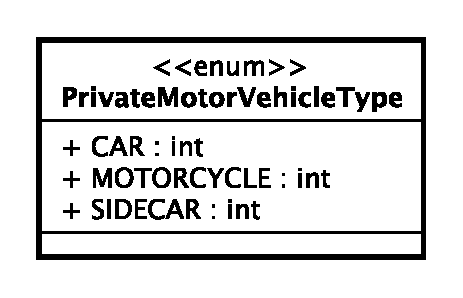
\includegraphics[scale=0.6,keepaspectratio]{images/solution/app/backend/private_motor_vehicle_type.eps}
\caption{\pReactiveComponentStretchDecoration::PrivateMotorVehicleType}
\label{fig:sd-app-private-motor-vehicle-type}
\end{figure}
\FloatBarrier
\begin{itemize}
  \item \textbf{\descr} \\
    It represents the type of a private motor vehicle.
  \item \textbf{\values}
  \begin{itemize}
    \item[+] \texttt{CAR: int} \\
    A private motor vehicle that is a car.
    \item[+] \texttt{MOTORCYCLE: int} \\
    A private motor vehicle that is a motorcycle.
    \item[+] \texttt{SIDECAR: int} \\
    A private motor vehicle that is a sidecar.
  \end{itemize}
\end{itemize}